\documentclass[11pt,conference]{ieeeconf}
\bibliographystyle{ieeetr}
\usepackage{graphicx}
\usepackage{subcaption}
\usepackage{cite}
\usepackage{float}
\graphicspath{{/}}
\begin{document}
\title{Lensless Image Classification for Machine-based Decision Making}
\author{
\begin{tabular}[t]{c c}
Ganghun Kim & Brian Rodriguez\\
\small Department of Electrical and Computer Engineering & \small Department of Electrical and Computer Engineering\\ 
\small University of Utah & \small University of Utah
\end{tabular}
\\
\begin{tabular}[t]{c}
Rajesh Menon\\
\small Department of Electrical and Computer Engineering\\
\small University of Utah
\end{tabular}
}
\maketitle

\abstract
Deep Learning (DL) has accelerated advancements in Image Classification via convolutional neural networks (CNNs). However, these image classification tasks have been widely trained on images taken with typical cameras; human-centric images. Here, we present a CNN trained using data taken by a single CMOS image sensor with no lens. We created a dataset of lensless images comprised of handwritten digits taken from the MNIST dataset. Then, we trained a CNN on this dataset and were able to show that for 10 digits, the CNN is able to classify lensless images with 96.6\% accuracy.
%
\section{Introduction}
Wide-scale deep learning algorithms have pushed image classification tasks to its limits. State of the art architectures have been able to classify human-centric images with astonishing accuracy, but human-centric images require expensive cameras \cite{DBLP:journals/corr/SimonyanZ14a, DBLP:journals/corr/SzegedyIV16}. Recently, lensless imaging has been gaining traction \cite{DBLP:journals/corr/AsifASVB15, Gill:13, DBLP:journals/corr/KimIPM17}. These lensless images are taken using a low cost and light-weight image sensor without the use of a camera lens. Previously, we demonstrated that machine learning algorithms can accurately classify lensless images for 2 digits with 99\% accuracy using support vector machines (SVMs) \cite{DBLP:journals/corr/abs-1709-00408}. Here, we extend this idea and use DL to classify lensless images for 10 digits, accurately. Moreover, we trained a CNN on a dataset of lensless images that we captured using a lensless camera.
%
\begin{figure}[H]
\centering
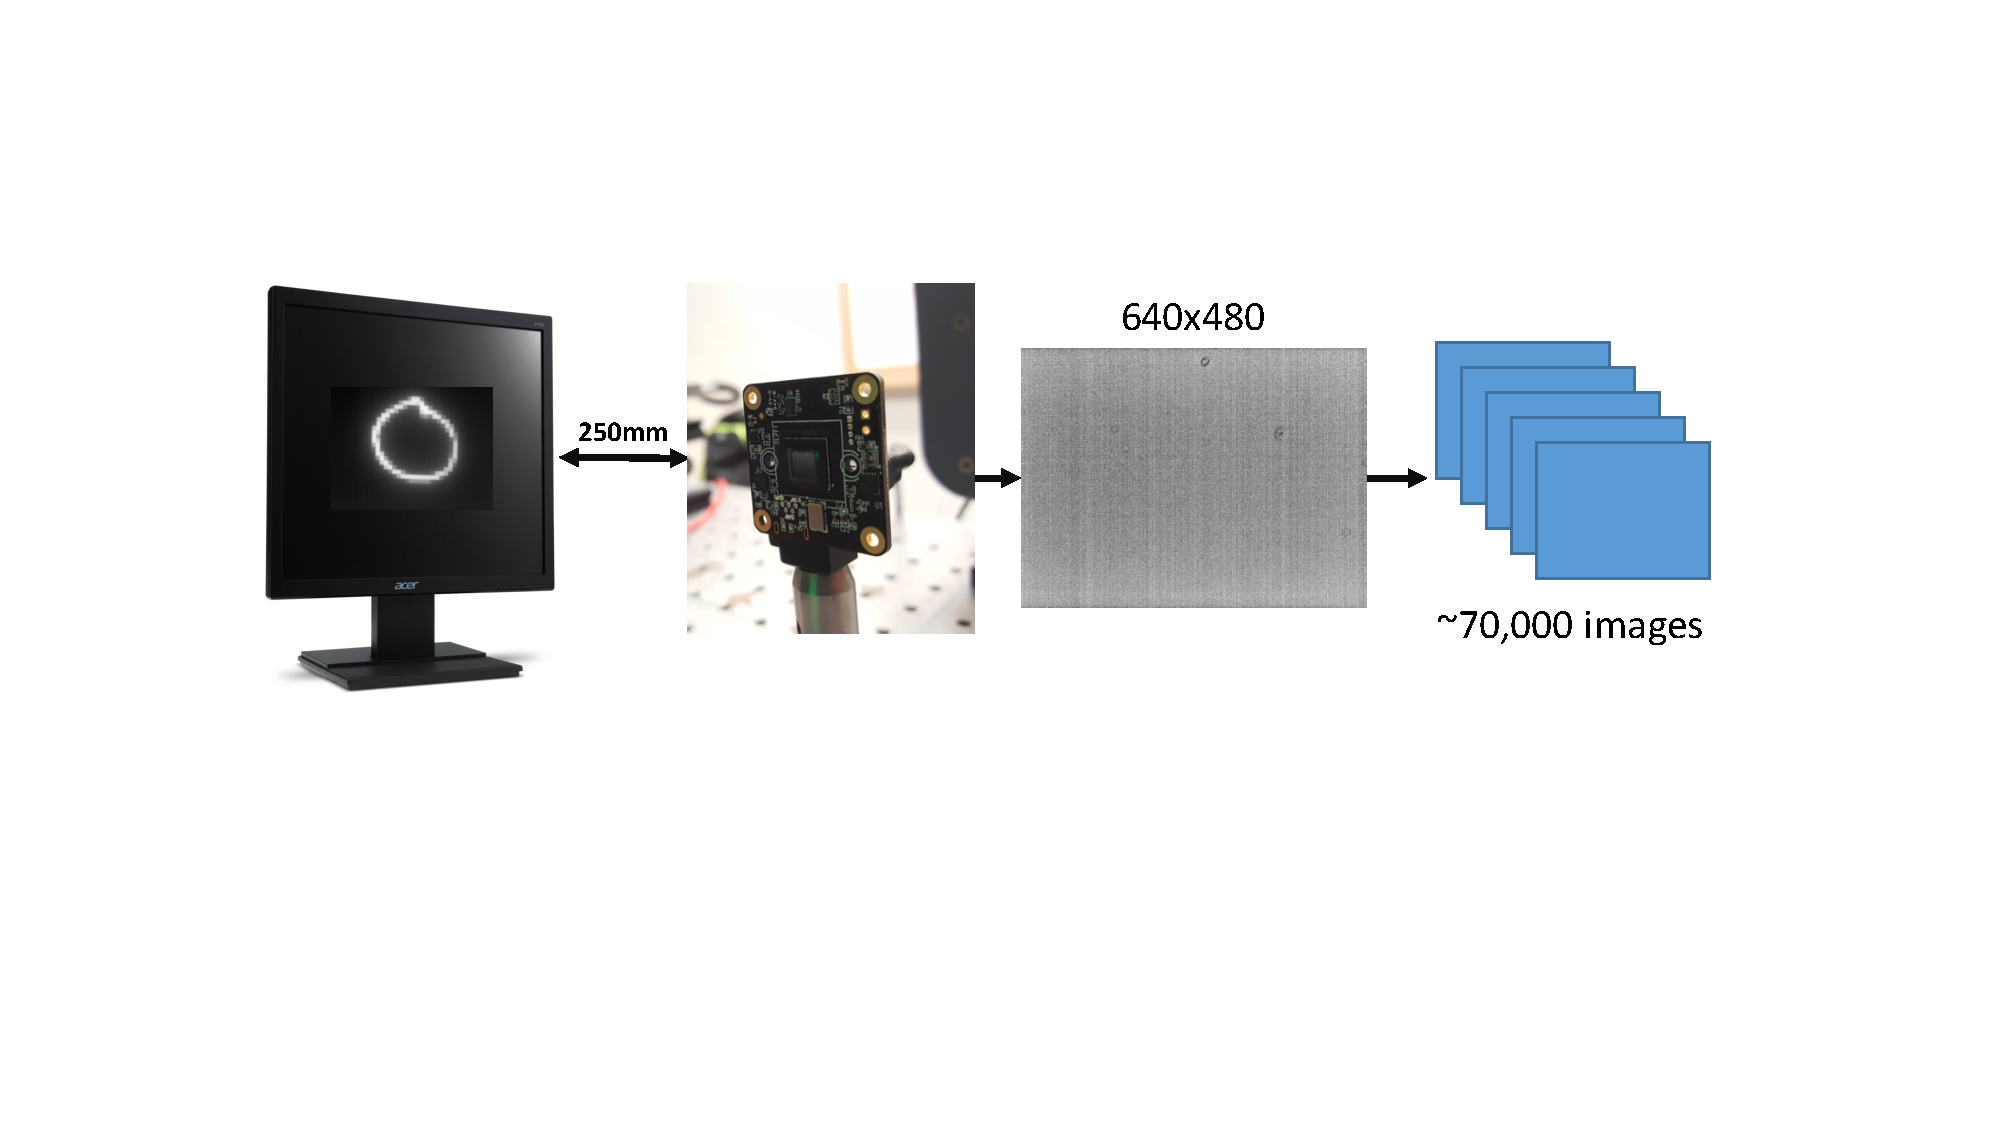
\includegraphics[keepaspectratio=true,scale=0.36]{imagingprocess}
\caption{}\label{section2_3}
\end{figure}
%
Our lensless camera consists of a simple CMOS image sensor. We used a liquid-crystal display (LCD) that displayed images of hand-written digits taken from the open-sourced MNIST dataset \cite{lecun-mnisthandwrittendigit-2010}. The LCD rests 250mm away from the CMOS sensor with an exposure time of 150ms and averaged over 100 frames to reduce noise. Using this procedure, we captured 70,000 lensless images and created a dataset with appropriate labels. These lensless images are 640x480 (307,200 pixels per image) which for scalability purposes are resized to 240x240.
%
Our results demonstrate that CNNs can accurately classify multiple classes of data taken directly from a lensless camera.
%
\section{Background}
%Convolutional neural networks have redefined 
%
\section{Network Architecture}
We propose a CNN architecture that is able to classify lensless images at a 96.6\% accuracy. Our architecture is comprised of two main sections; feature section and a classifying section. The feature section has 4 subsections containing convolutional layers and max pooling layers. Each convolutional layer is followed by batch normalization and a ReLU activation function \cite{DBLP:journals/corr/IoffeS15, Nair:2010:RLU:3104322.3104425}.
\begin{figure}[H]
\centering
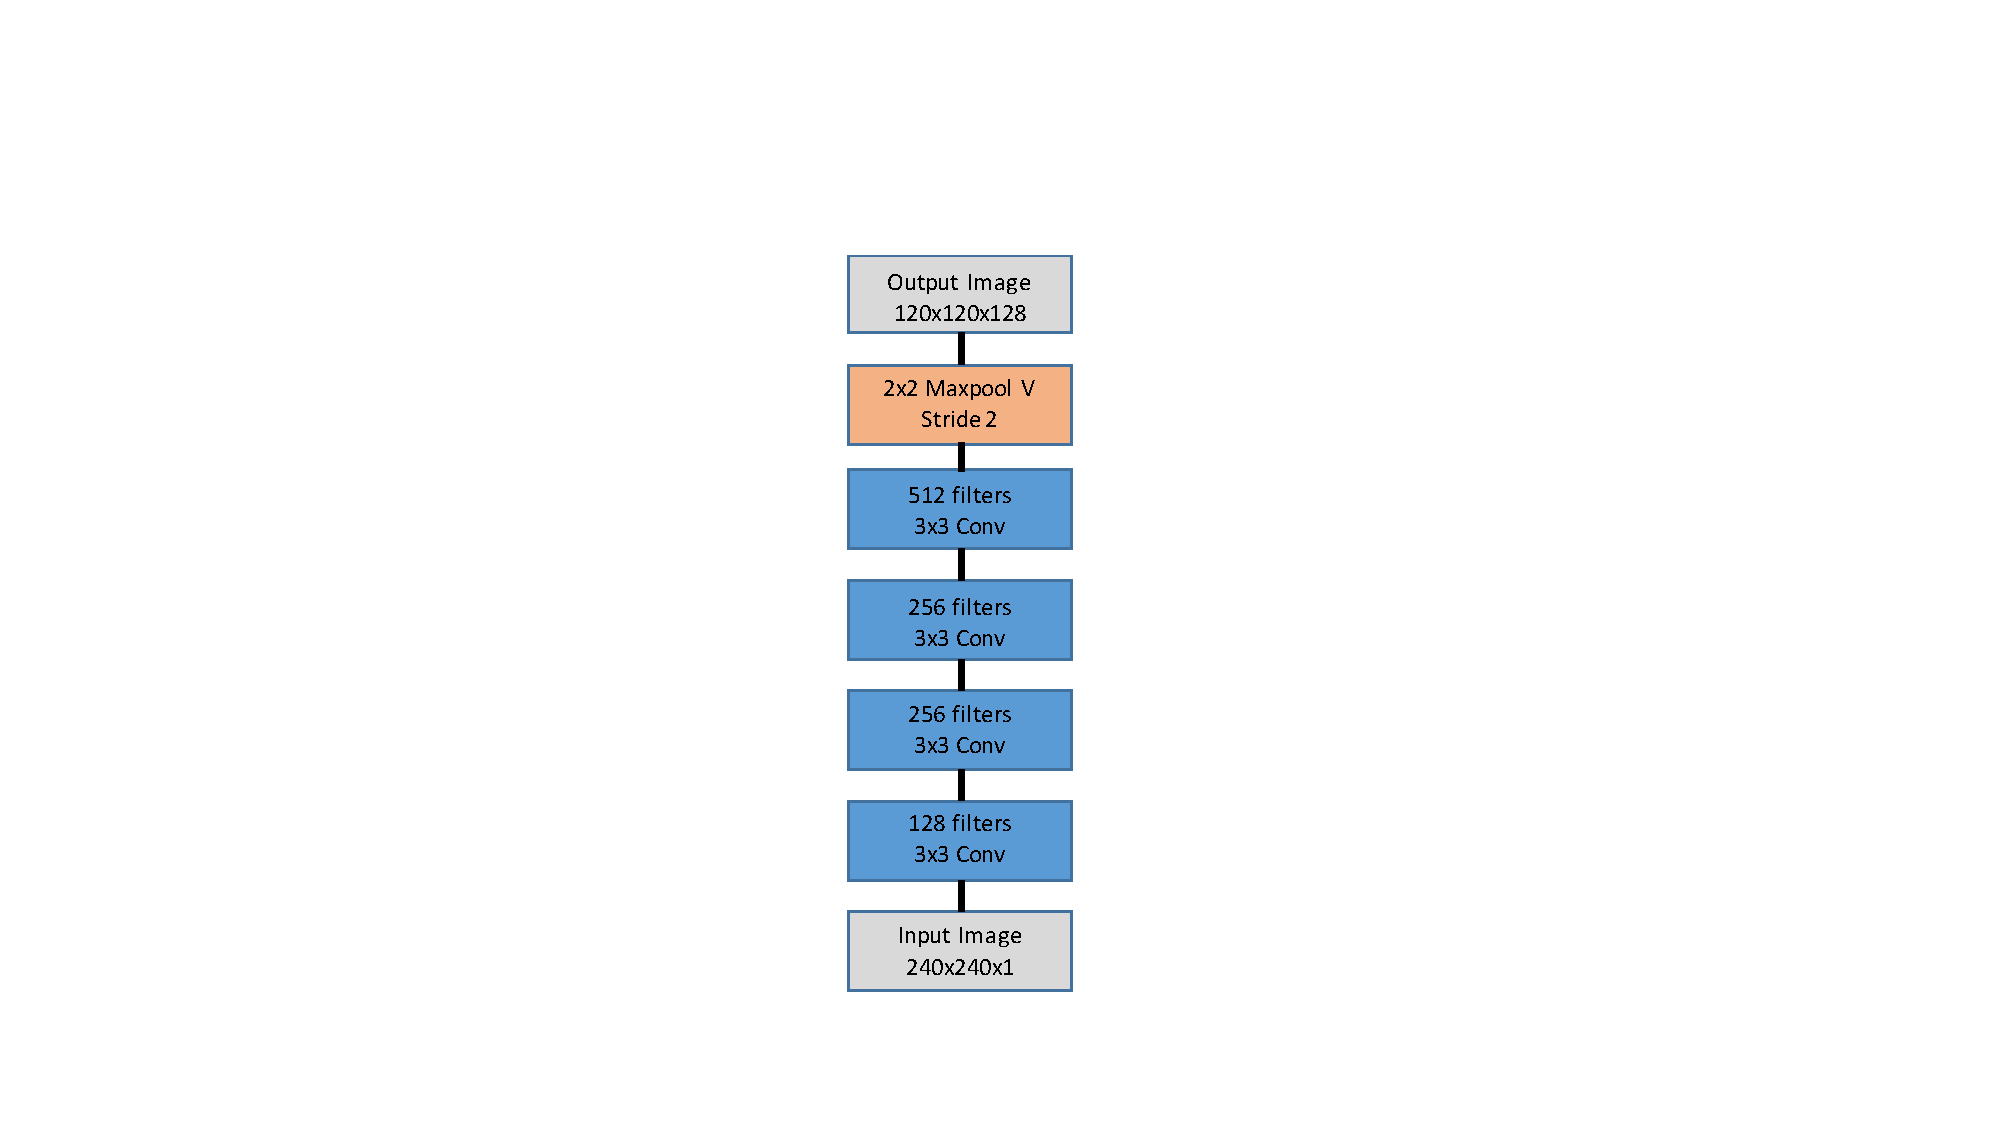
\includegraphics[keepaspectratio=true,scale=0.6]{section1}
\caption{Section 1 of the Convolutional Neural Network. Input images are sized to 240x240 and gray-scaled.}\label{section1}
\end{figure}
 The 1x1 convolutional layers are used for dimensionality reduction, these layers follow every pooling layer except for the last \cite{DBLP:journals/corr/LinCY13}. The 1x1 convolutions allowed for our network to converge faster.
% The 1x1 convolutional layers are a special case to this rule. These 1x1 layers are used for dimensionality reduction and do not utilize batch normalization or a ReLU activation function. 
Following the feature section is a classifying section. This section contains two fully-connected layers, where the last fully-connected layer classifies between the 10 different classes. We also employ dropout with a probability of .5 to prevent overfitting in the network \cite{JMLR:v15:srivastava14a}.
%
\begin{figure}[H]
\centering
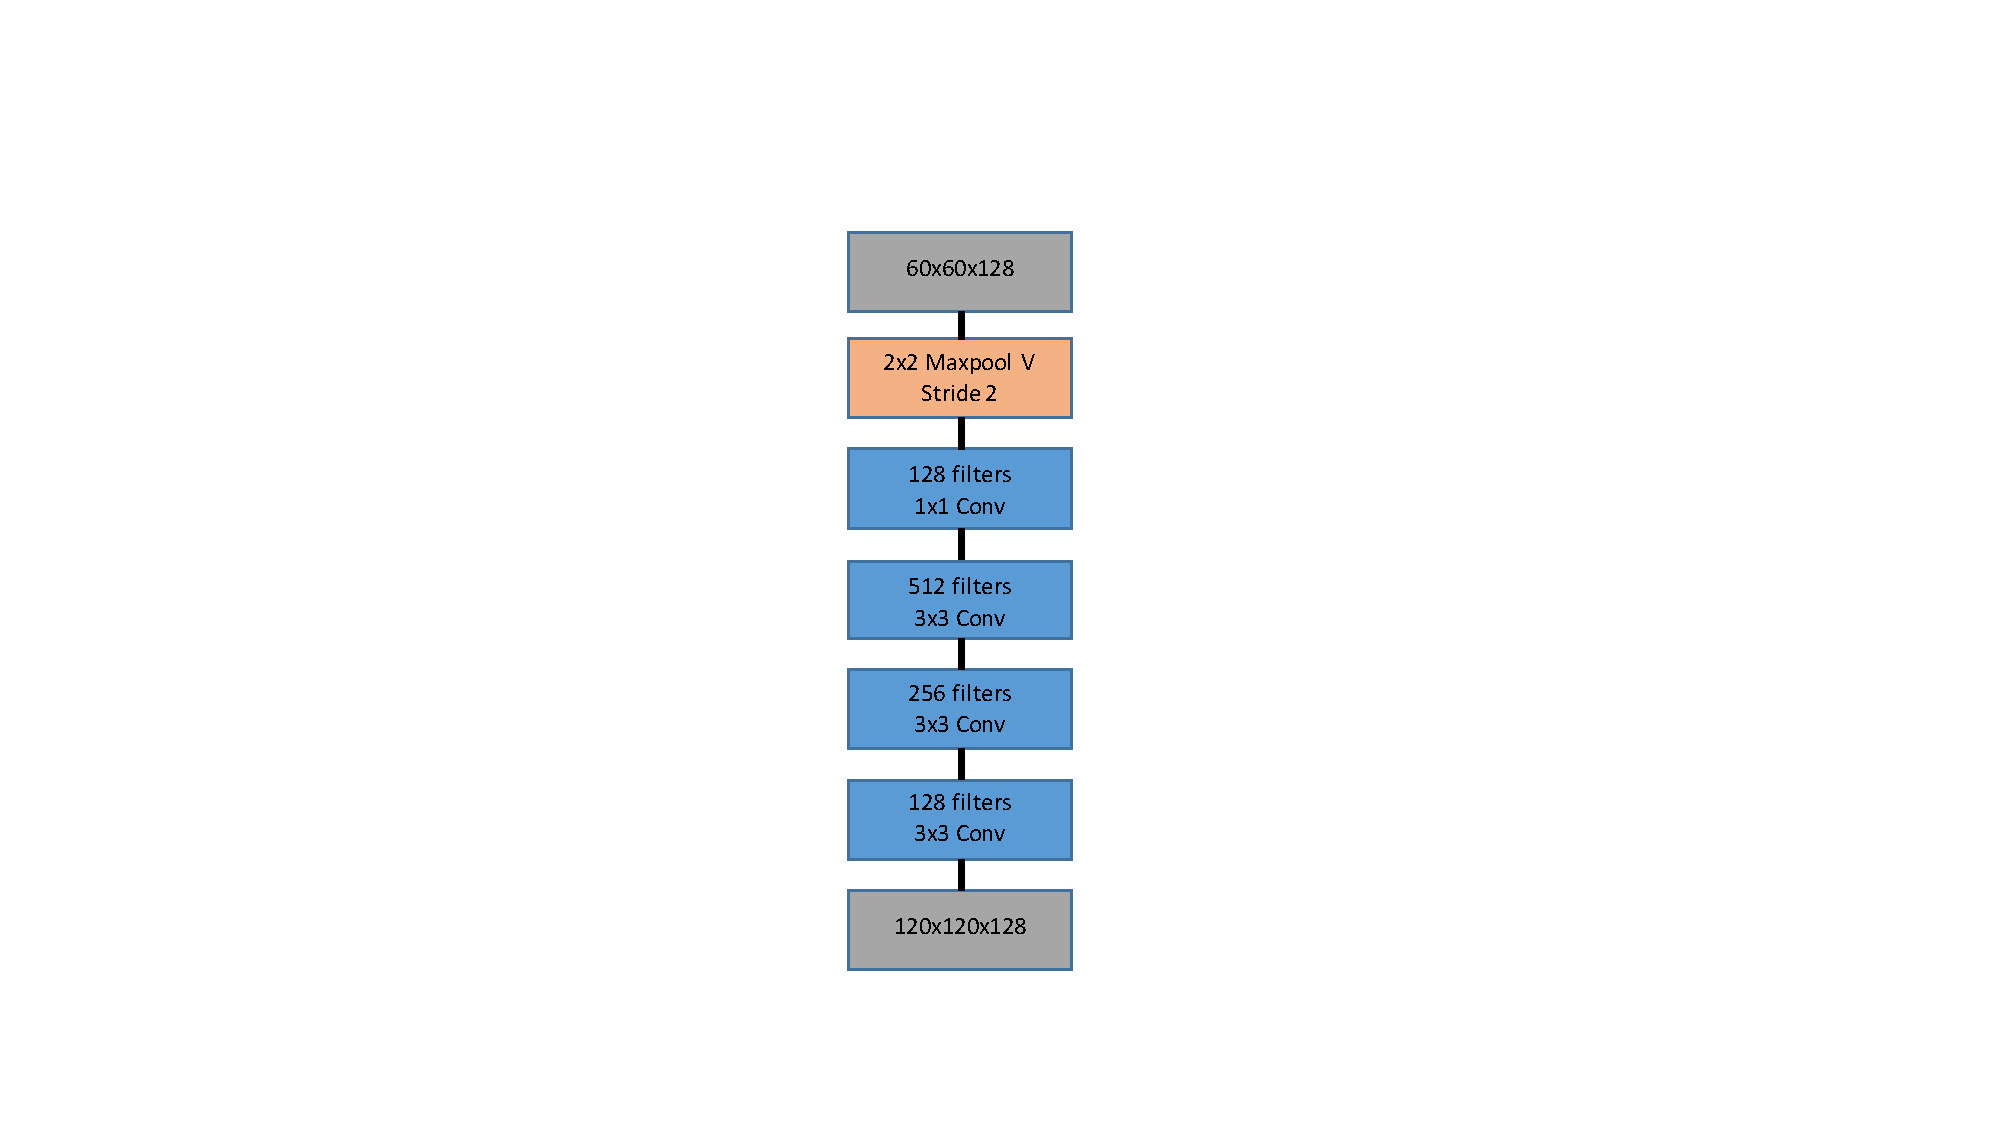
\includegraphics[keepaspectratio=true,scale=0.6]{section2}
\caption{Section 2 (Left) and Section 3 (Right) of the network. These two sections are identical except for their output dimensions of the images.}\label{section2_3}
\end{figure}
%
\begin{figure}[H]
\centering
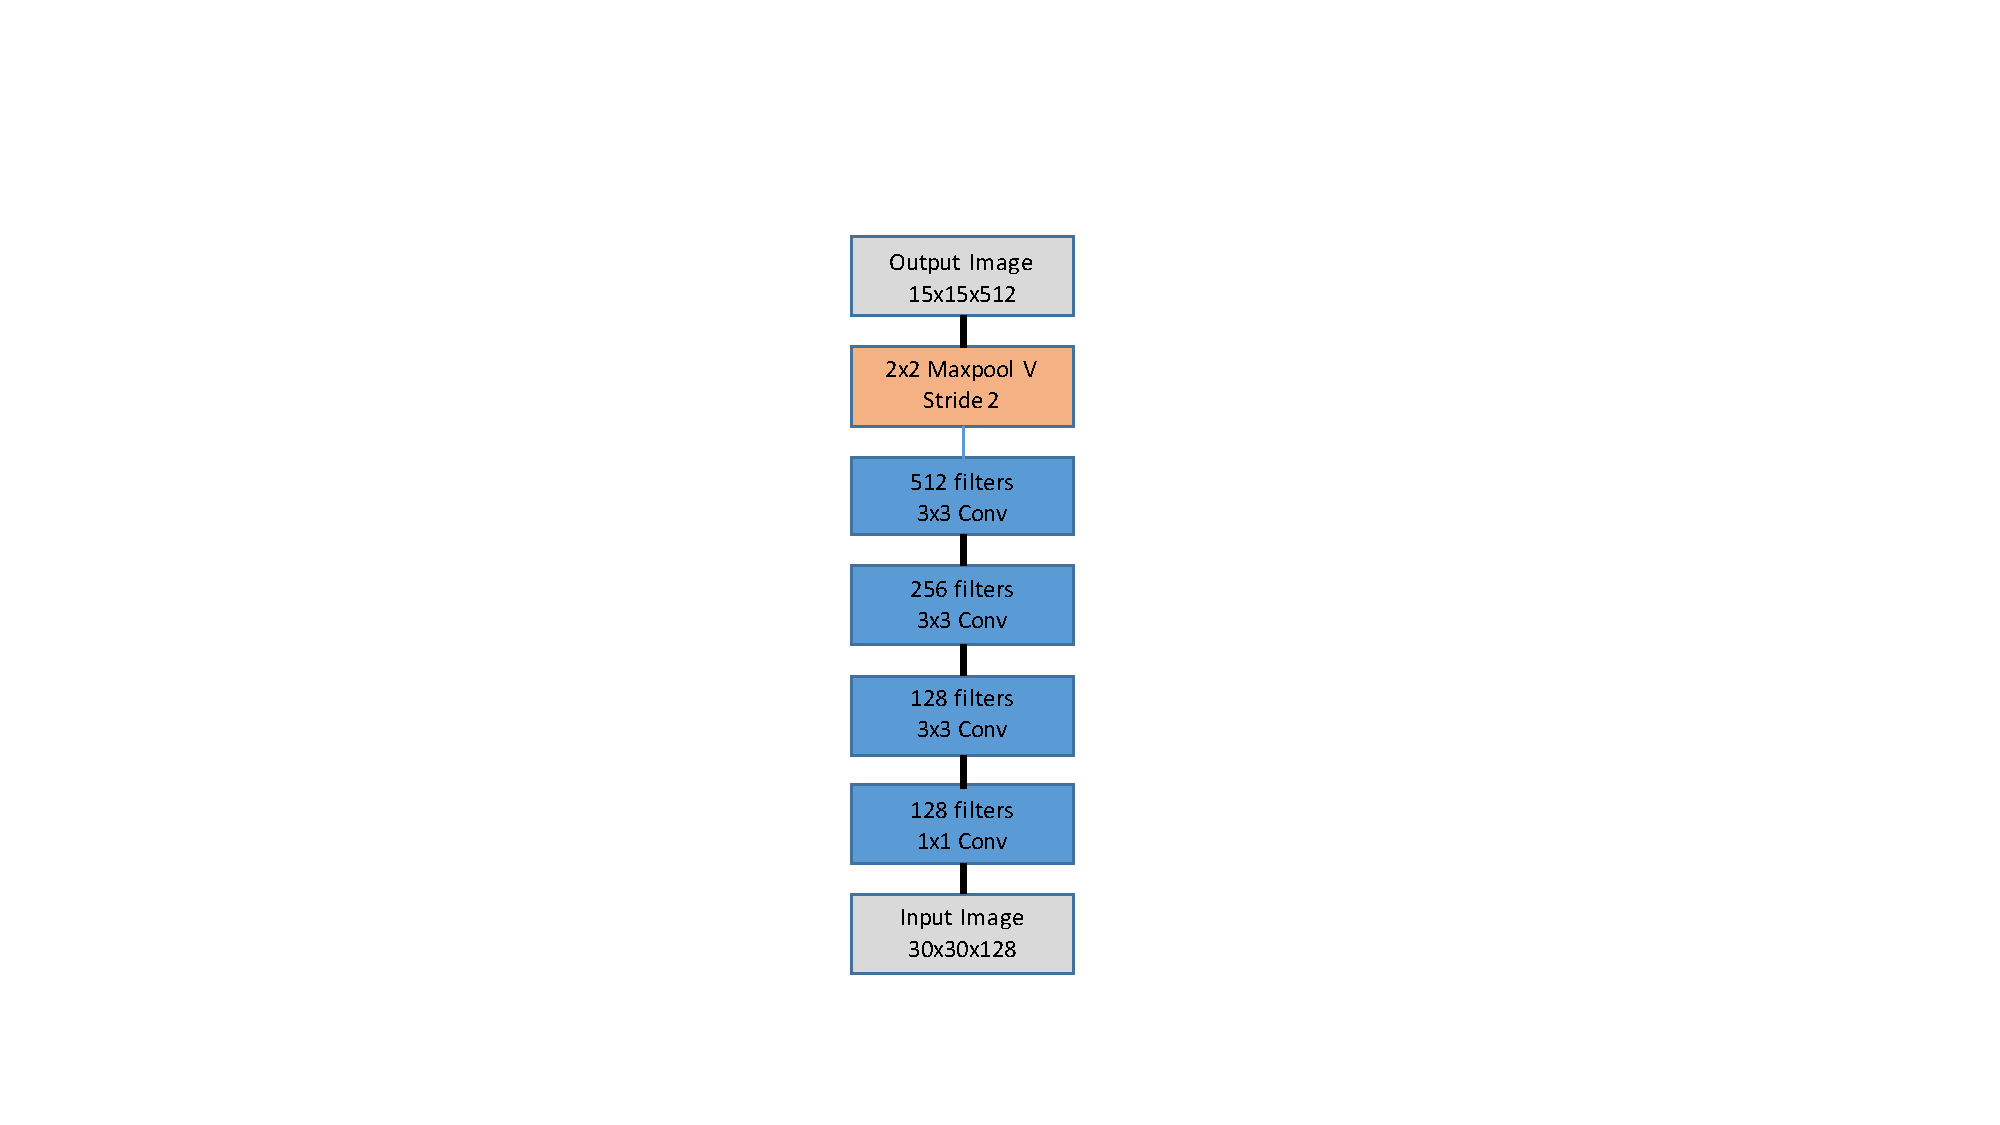
\includegraphics[keepaspectratio=true,scale=0.6]{section4}
\caption{Final feature section (Left) and the classification section (Right) of the network.}\label{section2_3}
\end{figure}
%
\section{Training Methodology}
We created our network using Pytorch, a highly extensible deep learning framework \cite{paszke2017automatic}. Our network was trained using stochastic gradient descent with a momentum of .9 on a single NVidia Tesla V100 GPU \cite{DBLP:journals/corr/KingmaB14, Sutskever:2013:IIM:3042817.3043064}. We used a learning rate of .001 and a mini-batch size of 16. The learning rate was decayed when the loss plateaued; decaying one time over 40 epochs. The input data is gray-scaled (by default) and the images are resized to 240x240. 5,400 images were taken from each class and split into two groups, training and testing groups; 3,200 training images and 2,200 testing images. Testing images are used for cross-validation; they serve to benchmark our model and test for overfitting in the network.
%
\section{Results}
%in our earlier trials
%While other gradient optimizers were tested such as Adam and Adagrad, they did not converge accordingly (ref)
We tested a lot of different configurations for our final network. Our earlier experimental networks actually saw the highest accuracy than some of our later networks. Our later networks employed ideas such as Alpha Dropout and SELU activation functions \cite{DBLP:journals/corr/KlambauerUMH17}. We noticed that using extra learnable parameters actually hindered our models ability to learn. The highest accuracy we found using these new methods of learning was 82\%. 
%
Our final network was able achieve a 96.6\% accuracy and converged in fewer epochs. Meaning, the network was able to learn the necessary features quicker, in less time. While other gradient optimizers were tested such as Adam and Adagrad they did not converge accordingly \cite{DBLP:journals/corr/KingmaB14, Duchi:EECS-2010-24}. We found that in all of our experiments, stochastic gradient decent was the best optimizer and allowed our network to converge to its global minimum.
%\section{Related Work}
%
%
\section{Conclusion}
Our results show promise for lensless imaging and a cost effective alternative for cameras in machine-based decision making.
%
\bibliography{biblio}

\end{document}